\documentclass[10pt,a4paper]{article}
\usepackage[margin=2.3cm]{geometry}
\usepackage{graphicx}
\usepackage{booktabs}
\usepackage{amsmath,amssymb}
\usepackage[font=small,labelfont=bf]{caption}
\usepackage[hidelinks]{hyperref}
\usepackage{xcolor}
\usepackage{float}
\usepackage[round]{natbib}
\usepackage[section]{placeins}
\newcommand{\NDone}{96}
\newcommand{\NQueue}{97}
\newcommand{\NLeft}{1}
\newcommand{\LaneHours}{107}
\newcommand{\NReal}{67}
\newcommand{\NRealEdge}{62}
\newcommand{\HoursLeft}{1}

\setlength{\parskip}{3pt}
\renewcommand{\topfraction}{0.9}\renewcommand{\bottomfraction}{0.8}\renewcommand{\textfraction}{0.07}\renewcommand{\floatpagefraction}{0.8}
\renewcommand{\arraystretch}{1.12}
\newcommand{\myr}{m\,yr$^{-1}$}
\newcommand{\mie}{m\,i.e.\,yr$^{-1}$}

\title{\textbf{Transient surface-mass-balance inversion with IGM\\for the ContinuIX intercomparison}\\[4pt]
\large Data, method and first results (GROUP\_UNIL, method01)}
\author{Kejdi Lleshi\\ \small Institute of Earth Surface Dynamics, University of Lausanne}
\date{\small Working document, 16 October 2026}

\begin{document}
\maketitle

\begin{abstract}
\noindent We describe our contribution to the ContinuIX intercomparison of continuity-based surface-mass-balance (SMB)
methods. The ice thickness is obtained by data assimilation of surface velocities, and of radar (GPR) thickness profiles
where they exist, through a convolutional-network emulator of ice flow; no provided thickness or bed field is used.
A one-dimensional SMB profile $b(z)$ is then inferred by differentiating a transient forward run through the
observation window. We summarise the twenty ContinuIX experiments, describe the synthetic glaciers and the data
coverage in detail, and report the results of \NDone\ of the \NQueue\ mandatory runs. On the steady-state synthetic
glacier S01 the inferred SMB matches the prescribed law with an RMSE of 0.67\,\mie\ ($R^2=0.95$), but the
flux divergence is biased by an overestimated thickness. On S02 the inferred thickness is unbiased to within
14\,m. Assimilating GPR profiles improves the fit to the assimilated profiles only; withheld profiles improve by
$\lesssim$\,3\,\%. The method fails on
grids coarser than about 100\,m on the synthetic glaciers. On the real glaciers G01 and G05 the thirteen perturbation
experiments change the glacier-wide SMB by at most 0.04\,\mie\ and the ELA by at most 43\,m. The raw, gappy data of EXP02 change the real-glacier results little (except on G06), but on S02, whose raw velocities
cover only the lower trunk, they lower the ELA by 500\,m. With globally available inputs
(EXP16--20) the glacier-wide SMB follows the global elevation-change product, and the global velocity product degrades
the inferred thickness. Runs with identical inputs differ by up to 0.22\,\mie\ through the L-curve choice of the
regularisation, which is the least reproducible step of the pipeline.
\end{abstract}

%=====================================================================================================================
\section{The ContinuIX intercomparison}

ContinuIX (\emph{Continuity approaches for mass-balance intercomparison}) is an IACS working group that compares methods
deriving distributed SMB from the continuity equation, $b = \partial h/\partial t + \nabla\!\cdot\!\mathbf{q}$, in
ice-equivalent units \citep{continuix}. All participants receive the same anonymised inputs (surface elevation DEM,
elevation change DHDT, surface velocity VX/VY, ice thickness THK, bed, glacier mask and uncertainties) and return SMB
and flux divergence (FDIV) with 1$\sigma$ uncertainties on the input grid. The organisers score the submissions against
withheld stake measurements of SMB and flux divergence and against glacier-wide geodetic balances.
Six real glaciers (G01--G06) and two synthetic glaciers (S01, S02) are used. Table~\ref{tab:exp} lists the twenty
experiments. EXP01 is the reference with homogenised, gap-filled inputs, and EXP02 provides the raw, gappy observations.
EXP03--15 perturb one input at a time on four mandatory glaciers (G01, G05, S01, S02), and EXP16--20 replace inputs by
globally available products. We run all mandatory glacier--experiment pairs, \NQueue\ runs in total.

\begin{table}[!htb]
\centering\small
\caption{ContinuIX experiments (WP2/WP3) and the glaciers run here.}
\label{tab:exp}
\begin{tabular}{lll l}
\toprule
ID & group & content & glaciers \\
\midrule
EXP01 & REF & homogenised, gap-filled data & G01--G06, S01, S02 \\
EXP02 & RAW & raw observations (gaps, several epochs, GPR points) & G01--G06, S02 \\
EXP03--07 & THK & perturbed thickness & G01, G05, S01, S02 \\
EXP08--13 & VEL & perturbed surface velocity & G01, G05, S01, S02 \\
EXP14--15 & RES & changed spatial resolution & G01, G05, S01, S02 \\
EXP16--20 & GLOB & globally available d$h$/d$t$, thickness and velocity products & G01--G06 \\
\bottomrule
\end{tabular}
\end{table}

%=====================================================================================================================
\section{Data}

\subsection{Glaciers}
Table~\ref{tab:glaciers} summarises the eight glaciers. The inputs are block-averaged to a model grid of 100\,m (50\,m
for glaciers smaller than 5\,km$^2$), which matches the resolution range of the ice-flow emulator. The thickness data
differ in kind. For G02, G03 and G05 the raw EXP02 package contains GPR survey points along profiles. For G01, G04 and
G06 it contains gridded thickness products covering 97--99\,\% of the glacier, which are interpolations rather than
measurements and are therefore not used. S02 has 62 synthetic profile cells, and S01 has none.

\begin{table}[!htb]
\centering\small
\caption{Glaciers. Window = inversion period ($t_1$--$t_2$; a 10-yr window is assumed for the synthetic cases);
ice cells on the model grid; "seg." = number of connected GPR profile segments.}
\label{tab:glaciers}
\setlength{\tabcolsep}{4pt}
\begin{tabular}{llrrrrl}
\toprule
 & type & native $\Delta x$ (m) & window (yr) & model $\Delta x$ (m) & ice cells & thickness data \\
\midrule
G01 & ice cap (11 basins) & 25 & 2013--2023 & 100 & 83\,261 & gridded \\
G02 & mountain glacier & 25 & 2006--2013 & 50 & 780 & profiles (10 seg.) \\
G03 & mountain glacier & 20 & 2012--2021 & 100 & 1\,229 & profiles (48 seg.) \\
G04 & mountain glacier & 2 & 2021--2025 & 50 & 887 & gridded \\
G05 & mountain glacier & 10 & 2017.67--2023.64 & 100 & 7\,904 & profiles (147 seg.) \\
G06 & mountain glacier & 10 & 2006--2017 & 100 & 1\,672 & gridded \\
S01 & synthetic, steady state & 1 & 10 yr (assumed) & 50 & 822 & none \\
S02 & synthetic, transient & 100 & 10 yr (assumed) & 100 & 8\,174 & profiles (4 seg.) \\
\bottomrule
\end{tabular}

\end{table}

\subsection{Synthetic glaciers}
\textbf{S01} is a steady-state synthetic valley glacier generated with \emph{icepack}: a 5\,km long half-pipe with a surface slope of 0.25, Glen exponent $n=3$ and ice at
$-1\,^\circ$C. Its SMB is prescribed as
$b(z)=\min[\,0.01\,(z-2350\,\mathrm{m}),\,5\,\mathrm{m\,yr^{-1}}]$, i.e.\ an ELA of 2350\,m (file attributes), which
makes S01 the only case with a known SMB truth. The data are given on a 1\,m grid with complete coverage of every
variable. Surface speeds are smooth (mean 46\,\myr) and d$h$/d$t$ is zero everywhere (Fig.~\ref{fig:s01},
Table~\ref{tab:syndata}).

\textbf{S02} is an idealised Aletsch-type glacier (simulated with Elmer/Ice) in a transient state: 83\,km$^2$
on a 100\,m grid, with several tributaries feeding a long tongue (Fig.~\ref{fig:s02}). It thins at
$-0.42$\,\myr\ on average, thickness reaches 756\,m, and surface speeds reach 241\,\myr.
No SMB field is provided, so its results can be checked against the true thickness and against mass conservation
only. Both synthetic glaciers come with uncertainty fields for velocity, d$h$/d$t$ and thickness.

\begin{figure}[!htb]
\centering
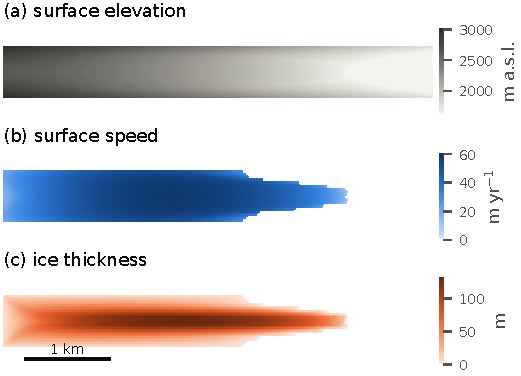
\includegraphics[width=0.75\textwidth]{figures/fig_s01_data.pdf}
\caption{S01 (EXP01): (a) surface elevation, (b) surface speed, (c) thickness. Ice flows from left to right;
d$h$/d$t$ = 0 (steady state).}
\label{fig:s01}
\end{figure}

\begin{figure}[!htb]
\centering
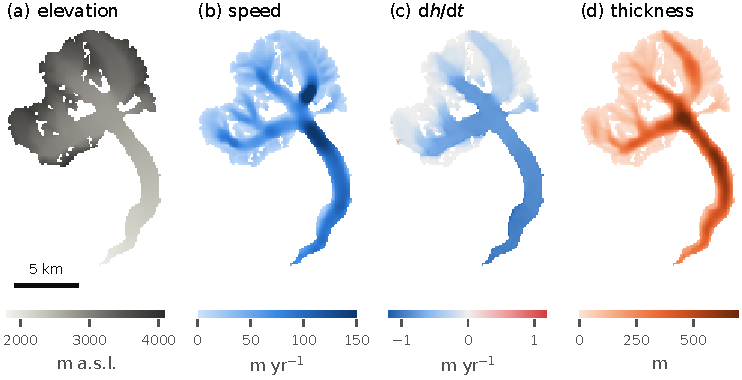
\includegraphics[width=\textwidth]{figures/fig_s02_data.pdf}
\caption{S02 (EXP01): (a) surface elevation, (b) surface speed, (c) elevation change, (d) thickness.}
\label{fig:s02}
\end{figure}

\begin{table}[!htb]
\centering
\caption{Synthetic inputs on the glacier (EXP01): resolution, area, value ranges, mean provided 1$\sigma$
uncertainties, and coverage of the glacier in EXP01 and in the raw data (EXP02).}
\label{tab:syndata}
\small\begin{tabular}{lrr}
\toprule
 & S01 & S02 \\
\midrule
grid spacing (m) & 1 & 100 \\
glacier area (km$^2$) & 2.03 & 82.68 \\
surface elevation (m a.s.l.) & 1604--2997 & 1850--4055 \\
surface speed mean / max (m yr$^{-1}$) & 46 / 59 & 48 / 241 \\
d$h$/d$t$ mean [range] (m yr$^{-1}$) & -0.00 [-0.00, +0.00] & -0.42 [-1.16, +0.42] \\
thickness mean / max (m) & 54 / 130 & 179 / 756 \\
$\sigma_{u}$ mean (m yr$^{-1}$) & 2.3 & 0.6 \\
$\sigma_{{\rm d}h/{\rm d}t}$ mean (m yr$^{-1}$) & 0.2 & 0.2 \\
$\sigma_{H}$ mean (m) & 8.1 & 2.5 \\
EXP01 coverage of $u_s$ / d$h$/d$t$ / $H$ (\%) & 100 / 100 / 100 & 100 / 100 / 100 \\
EXP02 coverage of $u_s$ / $H$ (\%) & n/a / n/a & 33.0 / 0.7 \\
\bottomrule
\end{tabular}

\end{table}

\subsection{Perturbation experiments}
The organisers do not describe the perturbations in detail, so Table~\ref{tab:pert} characterises them from the data,
relative to EXP01, for the four mandatory glaciers. The thickness experiments add random noise (EXP03--05; up to $\pm$46\,\% for the central 68\,\% of cells) or a
uniform $\pm$30\,\% bias (EXP06/07). The velocity experiments add noise in magnitude and direction (EXP08--12) or a positive speed bias (EXP13:
+13 to +44\,\%). The resolution experiments coarsen the grid (S01: 3\,m and 100\,m; S02: 300\,m, with
EXP15 identical to EXP01; G01: 75 and 100\,m; G05: 30 and 100\,m). Because our method uses no provided thickness field, the thickness experiments can
affect it only through the GPR observations. For S01 and G01, which have no GPR, EXP03--07 are formally identical to EXP01.

\begin{table}[!htb]
\centering\small
\caption{Perturbations relative to EXP01 (median $\pm$ half the 16--84\,\% range of the relative change; thickness on
cells $>$\,20\,m, speed on cells $>$\,5\,\myr).}
\label{tab:pert}
\resizebox{\textwidth}{!}{\begin{tabular}{lllll}
\toprule
 & S01 & S02 & G01 & G05 \\
\midrule
EXP03 & $H$: -1\,\% $\pm$ 24\,\% & $H$: -1\,\% $\pm$ 30\,\% & $H$: -0\,\% $\pm$ 30\,\% & $H$: -1\,\% $\pm$ 30\,\% \\
EXP04 & $H$: -4\,\% $\pm$ 17\,\% & $H$: -2\,\% $\pm$ 30\,\% & $H$: +2\,\% $\pm$ 29\,\% & $H$: -0\,\% $\pm$ 29\,\% \\
EXP05 & $H$: -0\,\% $\pm$ 7\,\% & $H$: +3\,\% $\pm$ 46\,\% & $H$: -0\,\% $\pm$ 18\,\% & $H$: +0\,\% $\pm$ 11\,\% \\
EXP06 & $H$: +30\,\% $\pm$ 0\,\% & $H$: +30\,\% $\pm$ 0\,\% & $H$: +30\,\% $\pm$ 0\,\% & $H$: +30\,\% $\pm$ 0\,\% \\
EXP07 & $H$: -30\,\% $\pm$ 0\,\% & $H$: -30\,\% $\pm$ 0\,\% & $H$: -30\,\% $\pm$ 0\,\% & $H$: -30\,\% $\pm$ 0\,\% \\
EXP08 & $|u_s|$: +2\,\% $\pm$ 7\,\% & $|u_s|$: -1\,\% $\pm$ 29\,\%, dir. $\pm$10.1$^\circ$ & $|u_s|$: +1\,\% $\pm$ 46\,\%, dir. $\pm$13.1$^\circ$ & $|u_s|$: -0\,\% $\pm$ 29\,\%, dir. $\pm$10.6$^\circ$ \\
EXP09 & $|u_s|$: +1\,\% $\pm$ 1\,\% & $|u_s|$: +1\,\% $\pm$ 33\,\%, dir. $\pm$7.4$^\circ$ & $|u_s|$: -0\,\% $\pm$ 22\,\%, dir. $\pm$6.3$^\circ$ & $|u_s|$: -0\,\% $\pm$ 7\,\%, dir. $\pm$3.9$^\circ$ \\
EXP10 & $|u_s|$: +0\,\% $\pm$ 2\,\% & $|u_s|$: +1\,\% $\pm$ 10\,\% & $|u_s|$: -0\,\% $\pm$ 10\,\% & $|u_s|$: +0\,\% $\pm$ 10\,\% \\
EXP11 & $|u_s|$: -0\,\% $\pm$ 3\,\%, dir. $\pm$0.5$^\circ$ & $|u_s|$: -0\,\% $\pm$ 8\,\%, dir. $\pm$3.0$^\circ$ & $|u_s|$: +0\,\% $\pm$ 8\,\%, dir. $\pm$2.8$^\circ$ & $|u_s|$: +0\,\% $\pm$ 8\,\%, dir. $\pm$2.8$^\circ$ \\
EXP12 & $|u_s|$: -3\,\% $\pm$ 2\,\%, dir. $\pm$0.3$^\circ$ & $|u_s|$: +0\,\% $\pm$ 9\,\%, dir. $\pm$3.4$^\circ$ & $|u_s|$: -0\,\% $\pm$ 5\,\%, dir. $\pm$1.4$^\circ$ & $|u_s|$: +1\,\% $\pm$ 2\,\%, dir. $\pm$0.8$^\circ$ \\
EXP13 & $|u_s|$: +13\,\% $\pm$ 5\,\% & $|u_s|$: +44\,\% $\pm$ 53\,\% & $|u_s|$: +22\,\% $\pm$ 18\,\% & $|u_s|$: +14\,\% $\pm$ 25\,\% \\
EXP14 & resolution 1 $\rightarrow$ 3 m & resolution 100 $\rightarrow$ 300 m & resolution 25 $\rightarrow$ 75 m & resolution 10 $\rightarrow$ 30 m \\
EXP15 & resolution 1 $\rightarrow$ 100 m & identical to EXP01 & resolution 25 $\rightarrow$ 100 m & resolution 10 $\rightarrow$ 100 m \\
\bottomrule
\end{tabular}
}
\end{table}

\subsection{Limited coverage}
Figure~\ref{fig:coverage} shows the glaciers whose raw data (EXP02) leave large parts of the glacier unobserved. In S02
the velocities cover only the lower trunk (33\,\% of the glacier), and the thickness exists on 62 cells (0.7\,\%) along
four profile segments. Real GPR covers 1.5--6.9\,\% of the cells (G02, G03, G05). Raw velocities miss two thirds of G04
and one third of G06. Velocity-free cells carry no velocity misfit in the data assimilation (DA), so the thickness there
is constrained only by regularisation and by the flow of the observed parts.

\begin{figure}[!htb]
\centering
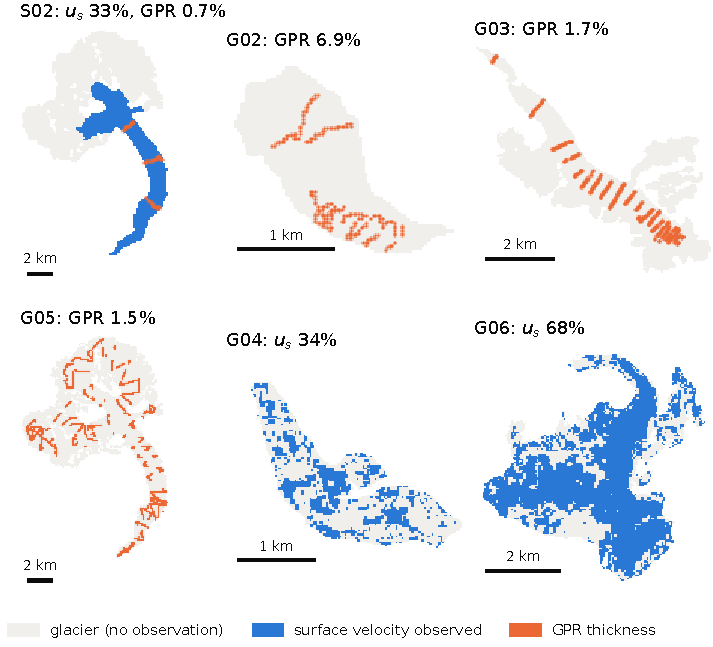
\includegraphics[width=0.8\textwidth]{figures/fig_coverage.pdf}
\caption{Raw-data coverage (EXP02, EXP01 grids). Gray: glacier without observation; blue: observed surface velocity
(shown where velocity is incomplete); orange: GPR thickness points. G04 and G06 have gridded thickness (98--99\,\%),
which is not shown.}
\label{fig:coverage}
\end{figure}

%=====================================================================================================================
\section{Method}

The method is the transient inversion of \citet{lleshi}, implemented in IGM \citep{igm}. Each glacier--experiment pair
is processed by the same automatic pipeline, which has no glacier-specific tuning.

\textbf{Ice-flow model.} IGM (development branch) with its pretrained convolutional emulator of the higher-order
equations, \texttt{pinnbp\_10\_4\_cnn\_16\_32} (10 vertical levels; inputs: thickness, surface, rate factor $A$,
sliding coefficient $\tau_{\rm ref}$, grid spacing).

\textbf{Data assimilation.} The thickness $H$ at the velocity epoch $t_{\rm DA}$ minimises
\begin{equation}
J(H)=\sum_{\rm vel}\frac{|\mathbf{u}_s(H)-\mathbf{u}_s^{\rm obs}|^2}{\sigma_u^2}
+\sum_{\rm GPR,\,assim.} w\,\frac{(H-H^{\rm obs})^2}{\sigma_H^2}+\lambda\,R(H)+J_{\rm mask},
\end{equation}
where $R$ penalises thickness gradients and curvature, $w$ down-weights densely sampled profile points, and the GPR
term is present only where GPR exists. No provided thickness or bed field enters the inversion. The first guess is a
perfect-plasticity thickness $H_0=\tau_y/(f\rho g\sin\alpha)$ ($\tau_y=100$\,kPa, $f=0.8$) from the smoothed surface
slope. The two scalar flow parameters ($\tau_{\rm ref}\in[0.05,2]$\,MPa, $A\in[30,120]$\,MPa$^{-3}$\,yr$^{-1}$) are
chosen by a 30-trial Optuna search \citep{optuna} on the final velocity misfit.

\textbf{GPR observations.} The GPR values of an experiment are its own THK at the GPR pixels, moved to
$t_{\rm DA}$ with DHDT, so that the thickness perturbations of EXP03--07 reach the observations (EXP02: the raw radar
points, averaged per model cell).

\textbf{Weight of the GPR: withheld profiles.} The GPR term of $J$ needs an observation error $\sigma_H$, and the
regularisation a weight $\lambda$. Neither can be chosen from the fit to the assimilated profiles themselves. A
smaller $\sigma_H$ or a weaker $\lambda$ always lowers that misfit, until the inferred thickness reproduces the
measurement and picking errors of the radar lines and develops artefacts between them, i.e.\ until the GPR receives
more weight than its accuracy justifies. The velocity misfit cannot arbitrate either, because the surface velocity is
nearly insensitive to the thickness along a single radar line. We therefore use cross-validation, the standard way of
choosing a regularisation parameter in ill-posed inverse problems \citep{hansen}: some profiles are withheld from the
inversion and serve only to judge it. The GPR cells fall into three groups:
\begin{itemize}\setlength{\itemsep}{1pt}
\item \emph{assimilated profiles} (60\,\% of the cells): they enter $J$;
\item \emph{cross-validation profiles} (20\,\%): withheld from $J$. For every pair $(\lambda,\sigma_H)$, with $\lambda\in\{100,300,1000\}$ and
$\sigma_H\in\{10,20,40,80\}$\,m, the inferred thickness is compared with them.
Among the settings whose misfit to these profiles is within 5\,\% of the best (and whose velocity misfit is within
1.5$\times$ the best), we take the largest $\sigma_H$, i.e.\ the least weight on the GPR, then the largest
$\lambda$. If two settings predict the withheld profiles equally well, the extra weight on the GPR is not supported by
the data;
\item \emph{independent profiles} (20\,\%): withheld from $J$ and from every choice. Their misfit plays the role of an
independent radar survey, an honest estimate of the thickness error away from the assimilated lines. It is only
reported.
\end{itemize}
The groups are made of whole profile segments (8-connected GPR cells, fixed random seed), not of single points.
Points along one radar line are a few metres apart and their errors are strongly correlated, so withholding single
points would only test the interpolation along the line; withholding whole segments tests the thickness between
the lines, which is where the method has to work. With fewer than ten segments the split is 70/30\,\% with no
independent group (S02). Without GPR, $\lambda$ is taken at the corner of an L-curve.

\textbf{SMB inference.} On the assimilated bed, the surface is integrated from $t_1$ to $t_2$ with
$\partial H/\partial t=b(z_s)-\nabla\!\cdot(H\bar{\mathbf u})$ (explicit, CFL 0.2, $H\ge0$ imposed after adding $b$),
with the flux recomputed by the emulator at every step. The profile $b(z)$ (piecewise linear, 200\,m nodes) minimises
the misfit to the end-of-window surface plus a curvature penalty (weight 0.05), using reverse-mode differentiation and
L-BFGS. FDIV $=b-\partial H/\partial t$ is the window-mean modelled flux divergence, so mass is conserved by construction.

\textbf{Family and uncertainty.} Velocity alone does not separate thickness from sliding. All $\tau_{\rm ref}$ with a
velocity misfit $\le$\,1.5$\times$ the best are kept (at most five), and SMB and FDIV are the mean of this family.
$\sigma_{\rm SMB}$ and $\sigma_{\rm FDIV}$ combine in quadrature the family spread, the residual of the end-of-window
geometry within each 50\,m elevation band (what a single $b(z)$ cannot explain), and the provided d$h$/d$t$ uncertainty.

%=====================================================================================================================
\section{Results}
\NDone\ of the \NQueue\ runs are complete, for \LaneHours\ GPU-hours on two RTX\,4090 cards. Only EXP14 for G01 is missing
(Sect.~\ref{sec:open}). A run takes about 0.5\,h (S01, G04) to 2\,h (G01).

\subsection{S01: comparison with the known SMB}
The inferred profile reproduces the prescribed gradient (0.0105--0.0125\,yr$^{-1}$ against 0.010) and places the ELA at
2277--2284\,m, 70\,m below the truth (Fig.~\ref{fig:s01prof}a, Table~\ref{tab:oldnew}). The five family members agree
closely. The pixel-wise SMB has an RMSE of 0.67\,\mie\ ($R^2=0.947$), better than with the previous emulator
(SIADecompNet; 0.86, $R^2=0.913$). The flux divergence is worse, however. Without thickness observations the
assimilated thickness stays near the plasticity first guess (mean 98\,m against a true 54\,m), and with the
selected flow parameters the flow is too fast for this geometry. The modelled glacier therefore thins at
0.90\,\myr\ instead of being in balance, which biases FDIV by +1.0\,\mie. The earlier run looked better on thickness
only because it started from the provided (true) thickness, which the present method forbids.

\begin{figure}[!htb]
\centering
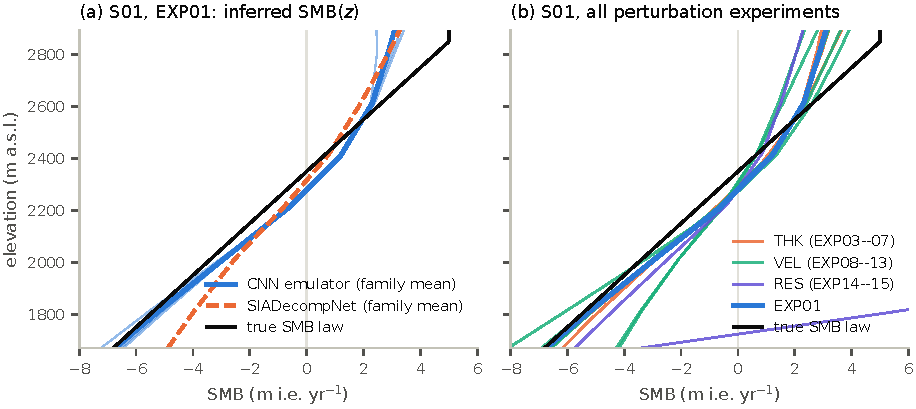
\includegraphics[width=\textwidth]{figures/fig_s01_profiles.pdf}
\caption{S01. (a) EXP01 SMB profile: family members (thin), family mean, previous emulator and the prescribed law.
(b) Family-mean profiles of all perturbation experiments. The outlier is EXP15 (100\,m grid), see Sect.~\ref{sec:sens}.}
\label{fig:s01prof}
\end{figure}

\begin{table}[!htb]
\centering\small
\caption{Synthetic glaciers, EXP01: present method (CNN emulator, no provided thickness, GPR) against the earlier
pipeline (SIADecompNet emulator, provided thickness as first guess). S02 has no SMB truth.}
\label{tab:oldnew}
\resizebox{\textwidth}{!}{\begin{tabular}{lrrrr}
\toprule
 & S01 CNN & S01 SIADecompNet & S02 CNN & S02 SIADecompNet \\
\midrule
pixel SMB RMSE (m i.e. yr$^{-1}$) & 0.67 & 0.86 & n/a & n/a \\
pixel SMB $R^2$ & 0.947 & 0.913 & n/a & n/a \\
ELA range of the family (m; true 2350) & 2277--2284 & 2171--2401 & -- & -- \\
glacier-wide SMB (m i.e. yr$^{-1}$) & -0.004 (true -0.138) & -0.040 & -0.169 & -0.193 \\
modelled / observed d$h$/d$t$ (m yr$^{-1}$) & -0.90 / -0.00 & -0.30 / -0.00 & -0.53 / -0.42 & -0.42 / -0.42 \\
FDIV RMSE vs true (m i.e. yr$^{-1}$) & 4.14 & 1.26 & n/a & n/a \\
thickness bias / RMSE (m) & +44 / 58 & -22 / 32 & +14 / 51 & -62 / 84 \\
thickness correlation & 0.70 & 0.93 & 0.97 & 0.98 \\
\bottomrule
\end{tabular}
}
\end{table}

\subsection{S01: what limits the SMB fit (twin experiment)}\label{sec:twin}
On S01 the SMB optimisation stops after 15 L-BFGS iterations, having lowered the data misfit (the RMS misfit of the
end-of-window thickness) by only 3\,\%, from 41.4 to 40.0\,m. To see whether the optimiser or the forward model is at
fault, we repeated the SMB step for one family member ($\tau_{\rm ref}=0.45$\,MPa) as a twin experiment. The observed
end-of-window surface is replaced by a forward run of our own model (same assimilated bed and thickness, same flow
parameters, same emulator) driven by the true S01 law, and the inversion starts from the same first-guess profile as
before. The target is thus consistent with the forward model by construction, and the answer is known.

In the twin experiment the misfit falls from 7.9 to 0.07\,m in 29 iterations, and the true law is recovered with a
profile RMSE of 0.05\,\mie, against 0.79\,\mie\ for the same member with the real observations
(Fig.~\ref{fig:twin}, pink; RMSE of the member's profile over 1669--2893\,m, not the pixel-wise family-mean value of
Table~\ref{tab:oldnew}). The optimiser, its gradients and the 200\,m profile basis are therefore not the limitation.
With the real observations the reverse holds: the true law, run through our forward model without iteration, gives a
misfit of 40.2\,m, slightly worse than the 40.0\,m reached by the inferred profile (Fig.~\ref{fig:twin}b, dashed).
Within this forward model the inferred profile explains the observations better than the true SMB does, so no
optimiser could do better.

The residual is a property of the forward model. Driven by the true SMB, the modelled glacier is not in steady state.
Within the ten-year window the first 150\,m of the glacier, where the assimilated thickness reaches 210\,m against the
domain edge, are emptied (partly by the border treatment, which removes ice within five cells of the domain edge), and
in the trunk the flanks thin by up to 43\,m while the centre thickens by up to 13\,m. Of the squared residual, 81\,\%
lies within 50\,m elevation bands, i.e.\ in a pattern that no profile $b(z)$ can represent. Because the inversion
closes $\partial H/\partial t=b-\nabla\!\cdot\mathbf q$ with the modelled flux, an error in the modelled flux
divergence is absorbed by $b$ where it projects onto elevation, and remains in the misfit where it does not. To first
order, the first part is the SMB error of Fig.~\ref{fig:twin}a and the second the misfit floor of
Fig.~\ref{fig:twin}b.

The SMB inference is therefore limited by the forward model as the data assimilation sets it up, i.e.\ by the emulator
run on the assimilated thickness and flow parameters, and not by the inversion itself. The twin experiment cannot tell
how much of the flux-divergence error comes from the ice-flow physics of the emulator (S01 was generated with
\emph{icepack}) and how much from the assimilated state, whose mean thickness is 98\,m against a true 54\,m because
the velocities alone do not separate thickness from sliding (Sect.~\ref{sec:open}). A forward run on the true S01
geometry would separate the two. The twin experiment is a verification of the method only: its observations are built
from the true SMB, which no real experiment provides, and it is not a result for any experiment.

\begin{figure}[!htb]
\centering
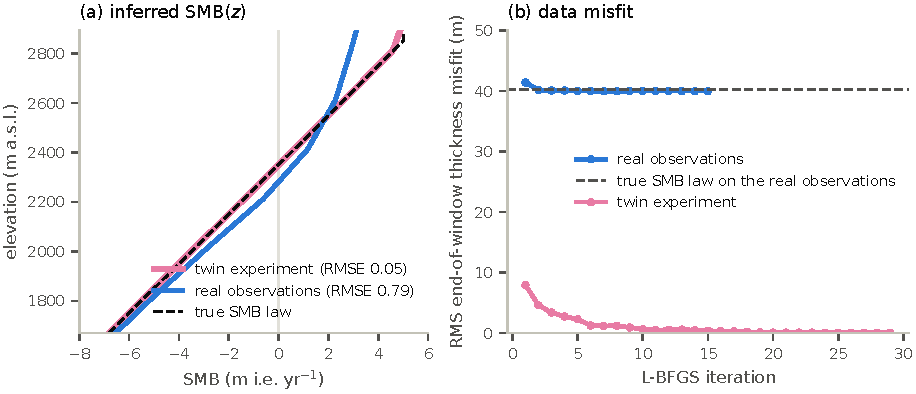
\includegraphics[width=\textwidth]{figures/fig_s01_twin.pdf}
\caption{S01 twin experiment, one family member ($\tau_{\rm ref}=0.45$\,MPa), SMB step of the submitted pipeline.
(a) SMB profile inferred from the real observations and from model-generated observations (twin experiment), against
the prescribed law; RMSE in \mie. (b) Data misfit per L-BFGS iteration. The dashed line is the misfit of the true law
on the real observations.}
\label{fig:twin}
\end{figure}

\subsection{S02 and the value of GPR}
On S02 the inferred thickness has a bias of +14\,m and an RMSE of 51\,m ($r=0.97$; Fig.~\ref{fig:s02thk}), against
$-62$ and 84\,m for the earlier pipeline. The thickness is underestimated along the main trunk and overestimated near the margins. The modelled thinning ($-0.53$\,\myr) slightly exceeds the observed one ($-0.42$\,\myr).

To isolate the effect of GPR we repeated the best DA without the GPR term, all else equal (Table~\ref{tab:gpr}). On S02,
GPR reduces the misfit at the assimilated cells from 70 to 27\,m but changes neither the misfit at the cross-validation
profile (52\,m) nor the whole-glacier error (51\,m). On G05 (147 segments, 683 assimilated cells) the misfit to the
independent profiles improves from 67 to 65\,m.
The profile information therefore remains local: the regularisation spreads it over a few cells, while the velocities
control the rest of the glacier. The cross-validation selected the weakest GPR weight ($\sigma_H=80$\,m on S02),
because stronger weights reduced the misfit at the assimilated cells to 2--3\,m without improving the fit to the
withheld profile.

Figure~\ref{fig:s02prof} shows which inputs matter. The top row plots, for every experiment, how much the input that
reaches our method was changed (horizontal axis) against how much the SMB profile moved away from EXP01 (vertical axis:
RMS difference over the glacier's elevation range, the same logarithmic axis in all three panels). The bottom row shows
the profiles themselves. The grey band marks the scatter between runs whose inputs are identical for our method
(0.06\,\mie), i.e.\ what the stochastic search of the flow parameters alone produces. The ranking is clear:
\begin{enumerate}\setlength{\itemsep}{1pt}
\item \textbf{resolution}: the 300\,m grid of EXP14 moves the profile by 11.6\,\mie, because the forward model fails;
\item \textbf{surface velocity}: the +44\,\% speed bias of EXP13 (1.8\,\mie) and the missing upper-glacier velocities of the
raw data (EXP02, 1.7\,\mie); random velocity noise matters less and depends on its kind: EXP09 (51\,\%
RMS change) moves the profile by 0.5\,\mie, EXP08 (44\,\%) by only 0.05;
\item \textbf{GPR thickness}: changing the assimilated GPR by 13--30\,\% moves the profile by at most
0.12\,\mie, barely above the scatter between repeated runs.
\end{enumerate}
In detail, the thickness experiments (EXP03--07) reproduce
the EXP01 profile (ELA 3125--3158\,m against 3156--3161\,m), as expected from the weak GPR weight. Among the velocity
experiments, the noise of EXP08 and EXP10--12 leaves the profile unchanged, EXP09 raises the ELA by 60\,m, and the
+44\,\% speed bias of EXP13 steepens the profile: 0.5--0.9\,\mie\ more negative below 3250\,m, up to 4.7\,\mie\ more
positive at the top, with the ELA 100\,m higher (3255\,m). EXP15 is identical
to EXP01. The 300\,m grid of EXP14 breaks the forward model (Sect.~\ref{sec:sens}), and its profile is inverted:
it decreases from +29\,\mie\ at the tongue to $-1.5$\,\mie\ at 3060\,m, so only its upper part falls inside the plotted range. Apart from that failure, the raw data of EXP02 change the profile most. With velocities on the lower trunk only, the
profile turns positive already at 2650\,m (ELA 2651--2660\,m, 500\,m below EXP01), peaks at +1.4\,\mie\ around 2900--3050\,m
and stays near zero above 3250\,m, where EXP01 reaches +1.5 to +2.7\,\mie. The glacier-wide SMB ($-0.13$ against
$-0.17$\,\mie) and the modelled thinning hardly change. The elevation distribution of the
SMB is therefore much less robust than its glacier-wide mean when large parts of the glacier lack velocity data.

\begin{figure}[!htb]
\centering
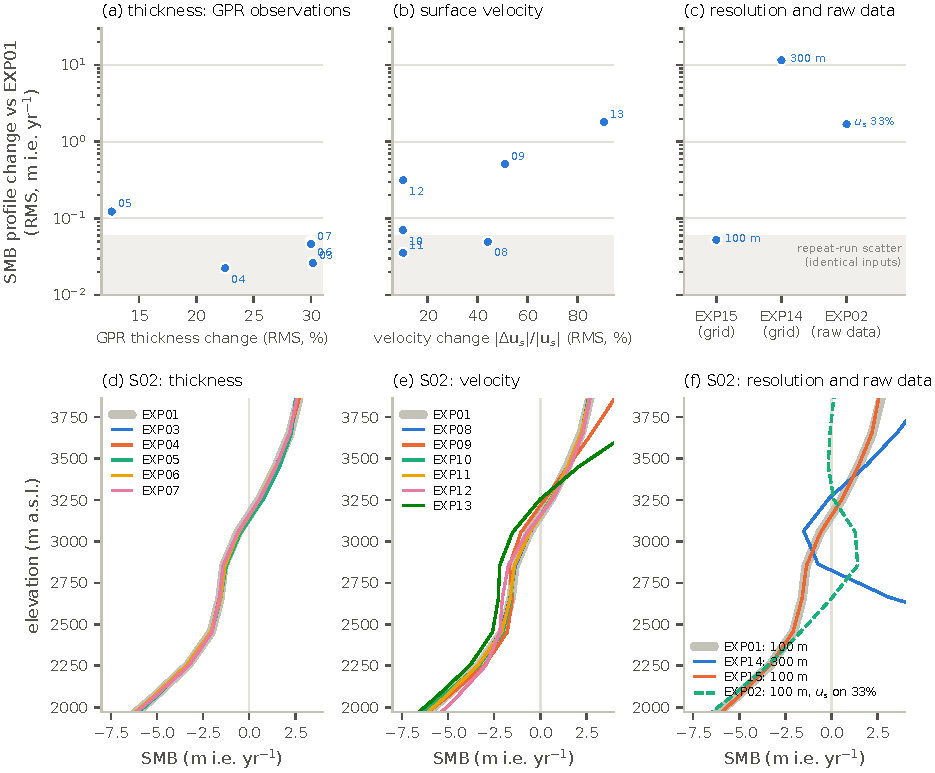
\includegraphics[width=\textwidth]{figures/fig_s02_profiles.pdf}
\caption{S02, sensitivity to the inputs. Top: change of the input that reaches the method, against the RMS change of the
SMB profile relative to EXP01 (common logarithmic axis; numbers = experiment). (a) Thickness experiments: RMS relative
change of the assimilated GPR thickness. (b) Velocity experiments: RMS of $|\Delta\mathbf{u}_s|/|\mathbf{u}_s|$ (magnitude,
direction and bias together). (c) Resolution and raw data, labelled with the model grid or the velocity coverage. Grey
band: scatter between runs with identical inputs. Bottom (d--f): family-mean SMB profiles, grouped likewise; EXP01 is the
wide grey line. The legend of panel (f) gives the grid spacing and, where incomplete, the fraction of ice cells with observed
surface velocity: EXP14 is on a 300\,m grid (forward model fails; profile off-scale below 2600\,m), EXP15 coincides with EXP01 (identical input), and EXP02
uses the EXP01 grid but has velocities on 33\,\% of the cells only.}
\label{fig:s02prof}
\end{figure}

\begin{figure}[!htb]
\centering
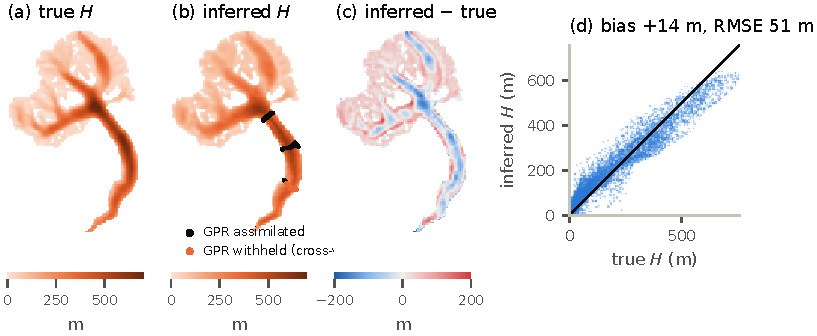
\includegraphics[width=\textwidth]{figures/fig_s02_thickness.pdf}
\caption{S02, EXP01: (a) true and (b) inferred thickness with the assimilated and the withheld (cross-validation) GPR cells, (c) difference,
(d) cell-by-cell comparison.}
\label{fig:s02thk}
\end{figure}

\begin{table}[!htb]
\centering\small
\caption{Effect of GPR in the DA (same $\tau_{\rm ref}$, $A$, $\lambda$): RMS thickness misfit (m) to the assimilated,
the cross-validation and the independent GPR profiles (Sect.~3), over the whole glacier against the true thickness (S02
only), and surface-velocity misfit. S02 has no independent profiles (four segments only).}
\label{tab:gpr}
\resizebox{\textwidth}{!}{\begin{tabular}{llrrrrr}
\toprule
glacier & DA & assimilated GPR & cross-validation GPR & independent GPR & whole glacier vs true $H$ & $u_s$ misfit (m yr$^{-1}$) \\
\midrule
S02 (EXP01) & with GPR & 27 & 52 & -- & 51 & 11.9 \\
S02 (EXP01) & without GPR & 70 & 52 & -- & 51 & 11.9 \\
G05 (EXP01) & with GPR & 47 & 65 & 65 & -- & 12.1 \\
G05 (EXP01) & without GPR & 69 & 67 & 67 & -- & 12.0 \\
\bottomrule
\end{tabular}
}
\end{table}

\subsection{Sensitivity to perturbations}\label{sec:sens}
The synthetic results are robust to the thickness and velocity perturbations (Fig.~\ref{fig:sens};
Table~\ref{tab:synall} in the appendix). For S01 the SMB RMSE stays between 0.54 and 1.29\,\mie\ across EXP03--14.
For S02 the glacier-wide SMB stays between $-0.15$ and $-0.18$\,\mie, except under the +44\,\% velocity bias of EXP13
($-0.10$). The raw data of EXP02, with velocities on the lower trunk only, raise the S02 thickness RMSE from 51 to
93\,m. The method fails at coarse resolution. On the 100\,m grid of S01 (EXP15) the glacier is five cells wide, and on
the 300\,m grid of S02 (EXP14) the spacing lies outside the emulator's training range. In both cases the forward run
misses the end-of-window geometry by about 90\,m, and the inferred SMB is unusable (+26.5 and +3.4\,\mie\ glacier-wide).

\begin{figure}[!htb]
\centering
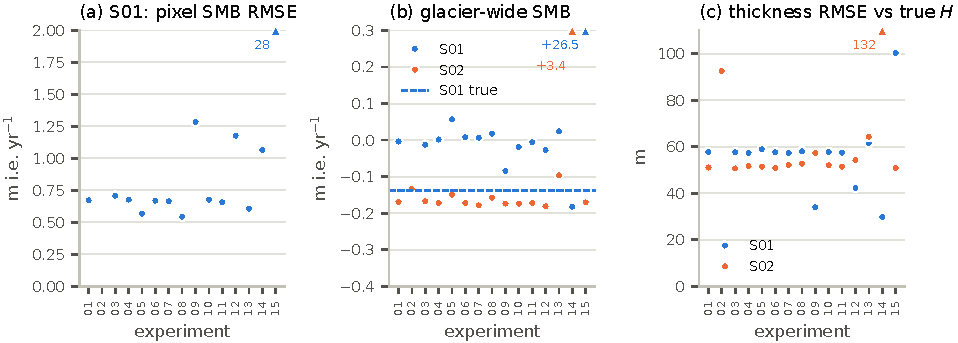
\includegraphics[width=\textwidth]{figures/fig_synthetic_sensitivity.pdf}
\caption{Synthetic glaciers across experiments: (a) S01 pixel SMB RMSE against the prescribed law, (b) glacier-wide
SMB, (c) thickness RMSE against the true thickness. Triangles: off-scale values (labelled).}
\label{fig:sens}
\end{figure}

\subsection{Real glaciers (EXP01)}
Figure~\ref{fig:real} and Table~\ref{tab:real} summarise the six real glaciers. Mass closure is good: the modelled
glacier-wide thinning matches the observed one within 0.1\,\myr\ for G01, G04, G05 and G06. G03 thins
0.31\,\myr\ too fast. G02 has a positive mean d$h$/d$t$ (+1.64\,\myr), which we consider doubtful (an open question to the
organisers). The ELAs are plausible. Where GPR exists, the RMS misfit of the
thickness to the independent profiles is 14\,m (G02), 51\,m (G03) and 65\,m (G05). Compared with the earlier emulator, the profiles agree in the
accumulation areas and differ mainly at the tongues, where the present method gives steeper ablation gradients
(G03, G06). The uncertainty is dominated by the elevation-band residual, not by the family spread
(Fig.~\ref{fig:g05}d).

\begin{figure}[!htb]
\centering
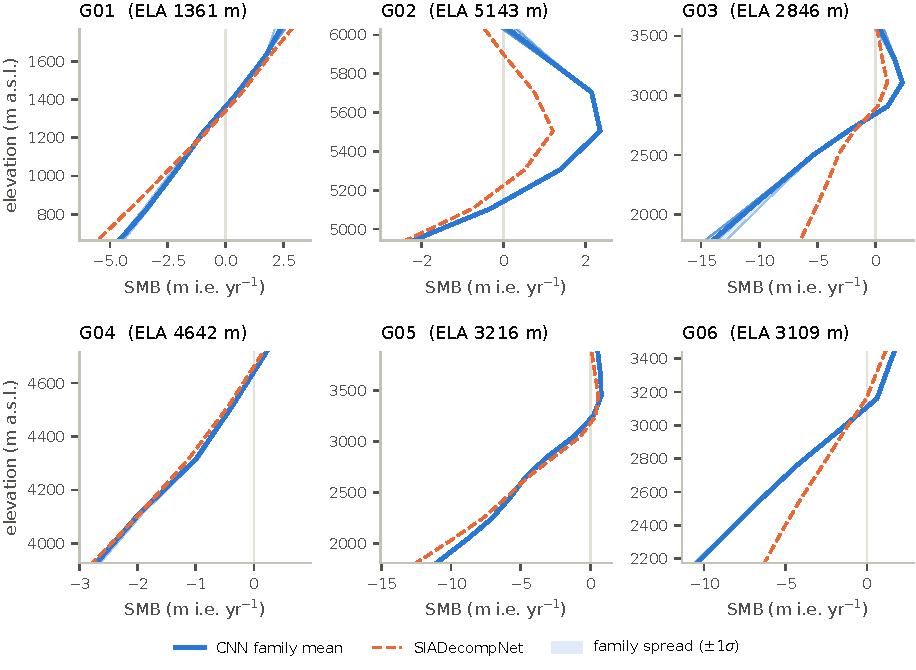
\includegraphics[width=\textwidth]{figures/fig_real_profiles.pdf}
\caption{Real glaciers, EXP01: inferred SMB profiles (family members, mean $\pm1\sigma$) and the earlier emulator.}
\label{fig:real}
\end{figure}

\begin{table}[!htb]
\centering
\caption{Real glaciers, EXP01. $\tau_{\rm ref}$ (MPa), $A$ (MPa$^{-3}$\,yr$^{-1}$),
velocity RMSE (mean observed speed) in \myr, mean DA thickness and RMS misfit to the independent GPR profiles (m), glacier-wide SMB, modelled
and observed mean d$h$/d$t$, mean FDIV, family-mean ELA (m), mean $\sigma_{\rm SMB}$, and the glacier-wide SMB of the
earlier pipeline (all \mie).}
\label{tab:real}
\resizebox{\textwidth}{!}{\begin{tabular}{lrrrrrrrrrrr}
\toprule
 & $\tau_{\rm ref}$ & $A$ & $u_s$ RMSE (mean) & $\overline{H}$ & indep. GPR & $\overline{\rm SMB}$ & $\overline{{\rm d}h/{\rm d}t}$ mod / obs & $\overline{\rm FDIV}$ & ELA & $\overline{\sigma}_{\rm SMB}$ & $\overline{\rm SMB}$ SIA \\
\midrule
G01 & 0.057 & 119 & 9.6 (25) & 147 & -- & -0.77 & -0.70 / -0.71 & -0.06 & 1361 & 1.15 & -0.82 \\
G02 & 0.071 & 119 & 3.9 (10) & 34 & 14 & +1.24 & +1.15 / +1.64 & +0.09 & 5143 & 1.20 & +0.30 \\
G03 & 0.115 & 119 & 9.3 (32) & 140 & 51 & -0.69 & -1.19 / -0.88 & +0.50 & 2846 & 2.83 & -0.68 \\
G04 & 0.333 & 30 & 2.6 (3) & 28 & -- & -1.29 & -1.21 / -1.30 & -0.08 & 4642 & 0.52 & -1.35 \\
G05 & 0.069 & 119 & 12.1 (41) & 161 & 65 & -1.93 & -2.04 / -1.95 & +0.11 & 3216 & 2.32 & -1.99 \\
G06 & 0.090 & 120 & 24.1 (31) & 117 & -- & -0.87 & -0.87 / -0.96 & +0.00 & 3109 & 1.71 & -0.80 \\
\bottomrule
\end{tabular}
}
\end{table}

\begin{figure}[!htb]
\centering
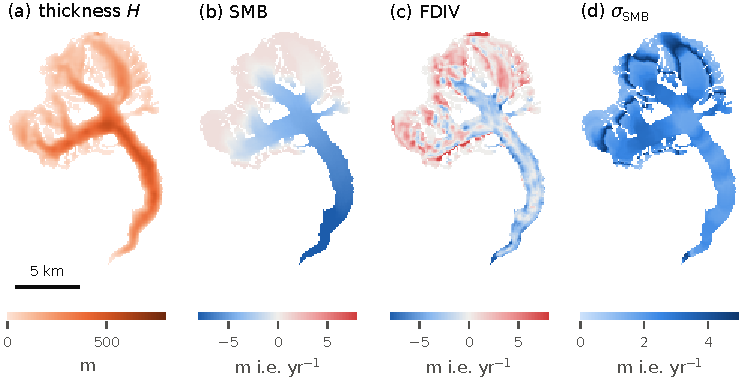
\includegraphics[width=\textwidth]{figures/fig_g05_maps.pdf}
\caption{G05, EXP01 (native grid): (a) assimilated thickness, (b) SMB, (c) flux divergence, (d) SMB uncertainty.}
\label{fig:g05}
\end{figure}

\subsection{Real glaciers under perturbation (G01, G05)}\label{sec:realsens}
On the two mandatory real glaciers the results hardly change across EXP03--15 (Fig.~\ref{fig:realsens},
Table~\ref{tab:realsens}). The glacier-wide SMB stays within 0.04\,\mie\ of EXP01 ($-0.77$ for G01, $-1.93$ for G05), and the
ELA stays within 14\,m, except for G05 on the 100\,m grid of EXP15 (+43\,m). This robustness is partly built in.
The glacier-wide flux divergence is small ($-0.06$ and +0.11\,\mie), so the glacier-wide SMB is essentially the mean observed d$h$/d$t$,
which the THK and VEL experiments do not change. The ELA and the distributed fields are the more telling quantities.
\begin{itemize}\setlength{\itemsep}{1pt}
\item \textbf{Thickness (EXP03--07).} For G01 these runs repeat EXP01. They differ only through the stochastic Optuna search, which returns
$\tau_{\rm ref}$ between 0.05 and 0.30\,MPa with practically the same SMB, an illustration of the sliding--thickness
equifinality. For G05 the perturbed GPR values enter the DA. The inferred thickness does not follow the +30\,\% bias
(EXP06: 161\,m as in EXP01) and follows the $-30$\,\% bias only partly (EXP07: 146\,m, $-9$\,\%). The noisy GPR of EXP03 and EXP04
lowers it by the same amount and raises the velocity misfit from 12 to 15\,\myr. The cross-validated choice of the GPR
weight therefore limits how much perturbed thickness data can leak into the result.
\item \textbf{Velocity (EXP08--13).} The noise of EXP08 ($\pm$46\,\% on G01) raises the velocity misfit (9.6 to 12.8\,\myr)
without changing the SMB. The +22\,\% (G01) and +14\,\% (G05) speed bias of EXP13 changes the mean thickness by +7 and $-6$\,m
and moves the ELA by 10--14\,m.
\item \textbf{Resolution (EXP14--15).} Unlike for the synthetic glaciers, the coarser grids do not break the method here,
because the real glaciers are already modelled on a 100\,m grid in EXP01: EXP15 only changes the input aggregation.
For G05, EXP15 makes the lower tongue up to 1\,\mie\ less negative. EXP14 for G01 (75\,m) has not run (Sect.~\ref{sec:open}).
\item \textbf{Raw data (EXP02).} The raw observations reproduce EXP01 closely on both glaciers: glacier-wide SMB $-0.78$
(G01) and $-1.90$\,\mie\ (G05), ELA within 11\,m. For G05 the raw GPR (corrected to the DEM epoch with the bed
elevation of the points) gives a misfit of 70\,m to the independent profiles, against 65\,m in EXP01.
\end{itemize}

The top row of Fig.~\ref{fig:realexpprof} ranks the inputs for the real glaciers as Fig.~\ref{fig:s02prof} does for S02.
On G01 only the speed bias of EXP13 (0.15\,\mie) rises clearly above the repeat-run scatter. On G05 the order differs
from S02: the coarse grid of EXP15 comes first (0.48\,\mie), then the GPR thickness (0.21--0.25\,\mie\ for EXP03, EXP04 and
EXP07, which thin the inferred ice), while the velocity perturbations stay at or below 0.11\,\mie. The GPR weighs more on
G05 than on S02 because it has 147 profile segments instead of four. The response to a thickness bias is asymmetric:
$-30$\,\% (EXP07) moves the profile by 0.25\,\mie, +30\,\% (EXP06) by 0.02. The SMB profiles (bottom rows) confirm this. For G01 every profile stays within
0.1\,\mie\ of EXP01 at all elevations, except EXP13, which is 0.3\,\mie\ more positive at the top. For G05 the profiles
stay within 0.3\,\mie, except where the inferred thickness changes: the thinner ice of EXP03, EXP04 and EXP07 makes the
tongue 0.4--0.5\,\mie\ less negative, and the coarse grid of EXP15 shifts it by up to 1.0\,\mie.

\begin{figure}[!htb]
\centering
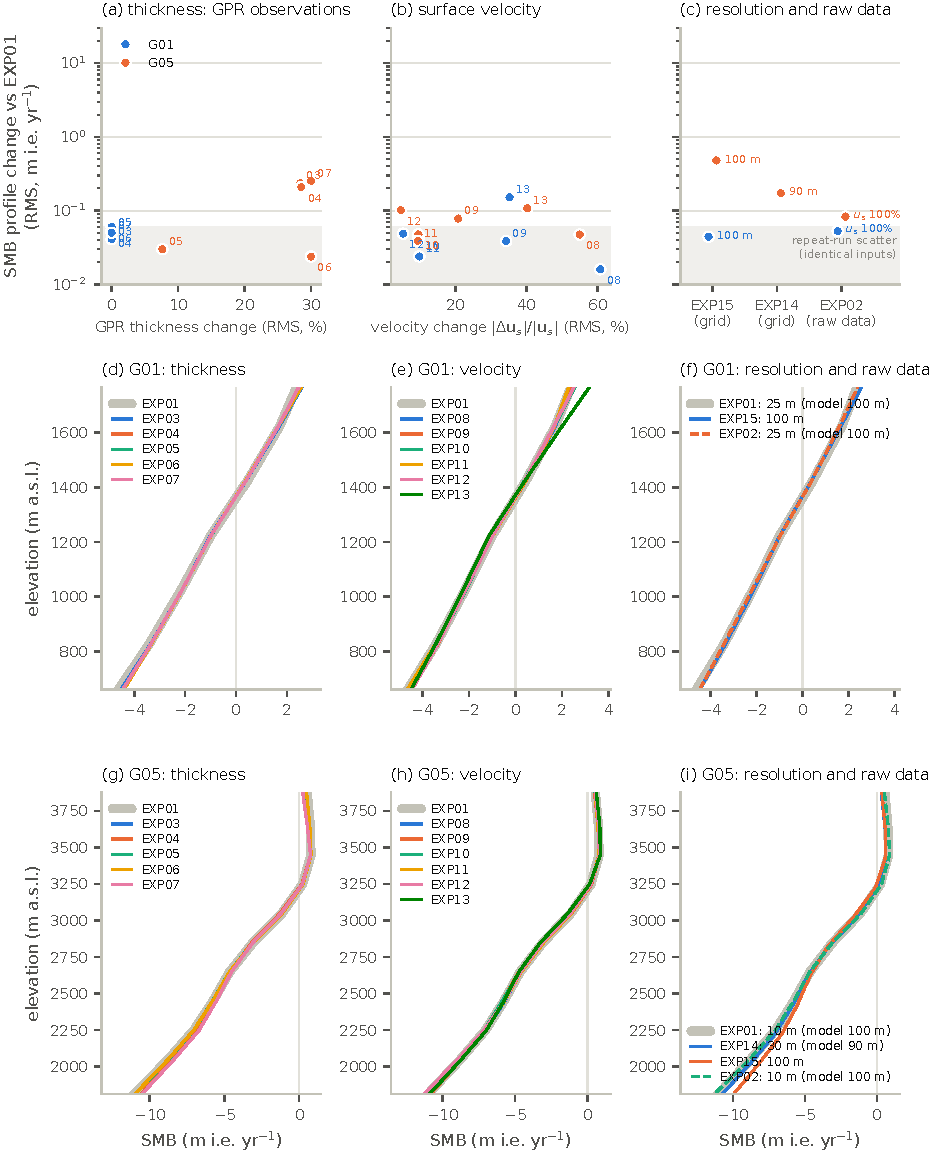
\includegraphics[width=\textwidth]{figures/fig_real_exp_profiles.pdf}
\caption{G01 and G05, sensitivity to the inputs. (a--c) As in Fig.~\ref{fig:s02prof}, for both glaciers (G01 has no GPR:
its thickness experiments are repeats of EXP01 and are plotted at zero change). (d--i) Family-mean SMB profiles of every
perturbation experiment and of the raw data (EXP02), grouped by type; EXP01 is the wide grey line. Right: native grid spacing and model grid of each run.}
\label{fig:realexpprof}
\end{figure}

\begin{figure}[!htb]
\centering
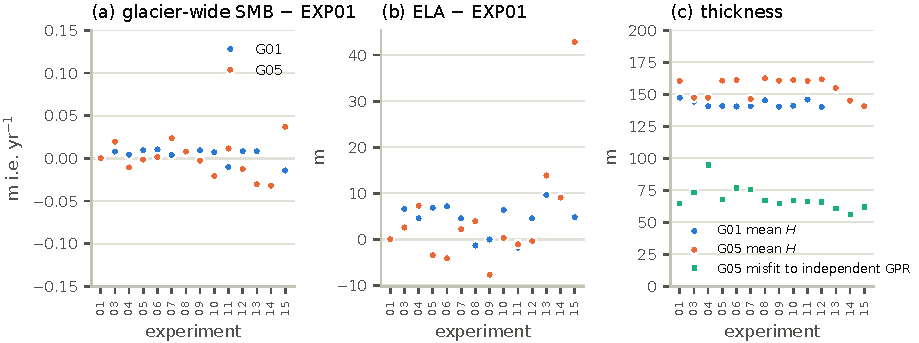
\includegraphics[width=\textwidth]{figures/fig_real_sensitivity.pdf}
\caption{Real glaciers G01 and G05 across the perturbation experiments: (a) glacier-wide SMB and (b) ELA relative to EXP01,
(c) mean inferred thickness and, for G05, the RMS misfit to the independent GPR profiles of each experiment (perturbed GPR in EXP03--07).}
\label{fig:realsens}
\end{figure}

\begin{table}[!htb]
\centering
\caption{G01 (left) and G05 (right) per experiment: native grid spacing (m), $\tau_{\rm ref}$ (MPa), velocity RMSE
(\myr), mean thickness (m), glacier-wide SMB (\mie), family-mean ELA (m) and, for G05, RMS misfit to the independent GPR profiles (m).}
\label{tab:realsens}
\resizebox{\textwidth}{!}{\begin{tabular}{l|rrrrrr|rrrrrrr}
\toprule
 & $\Delta x$ & $\tau_{\rm ref}$ & $u_s$ RMSE & $\overline{H}$ & $\overline{\rm SMB}$ & ELA & $\Delta x$ & $\tau_{\rm ref}$ & $u_s$ RMSE & $\overline{H}$ & $\overline{\rm SMB}$ & ELA & indep. GPR \\
\midrule
EXP01 & 25 & 0.06 & 9.6 & 147 & -0.77 & 1361 & 10 & 0.07 & 12.1 & 161 & -1.93 & 3216 & 65 \\
EXP03 & 25 & 0.05 & 9.7 & 144 & -0.76 & 1368 & 10 & 0.07 & 15.4 & 147 & -1.91 & 3218 & 73 \\
EXP04 & 25 & 0.30 & 9.6 & 141 & -0.76 & 1366 & 10 & 0.11 & 15.5 & 147 & -1.94 & 3223 & 95 \\
EXP05 & 25 & 0.30 & 9.6 & 141 & -0.76 & 1368 & 10 & 0.07 & 12.0 & 161 & -1.93 & 3212 & 68 \\
EXP06 & 25 & 0.06 & 9.6 & 141 & -0.76 & 1368 & 10 & 0.07 & 11.9 & 161 & -1.93 & 3212 & 77 \\
EXP07 & 25 & 0.30 & 9.6 & 141 & -0.76 & 1366 & 10 & 0.11 & 15.5 & 146 & -1.91 & 3218 & 76 \\
EXP08 & 25 & 0.07 & 12.8 & 145 & -0.76 & 1360 & 10 & 0.07 & 14.0 & 162 & -1.92 & 3220 & 67 \\
EXP09 & 25 & 0.08 & 10.2 & 140 & -0.76 & 1361 & 10 & 0.06 & 12.3 & 161 & -1.93 & 3208 & 65 \\
EXP10 & 25 & 0.05 & 10.2 & 141 & -0.76 & 1368 & 10 & 0.26 & 12.8 & 161 & -1.95 & 3216 & 67 \\
EXP11 & 25 & 0.99 & 9.9 & 146 & -0.78 & 1360 & 10 & 0.20 & 12.6 & 161 & -1.92 & 3215 & 66 \\
EXP12 & 25 & 0.07 & 9.7 & 140 & -0.76 & 1366 & 10 & 0.20 & 12.4 & 162 & -1.94 & 3215 & 66 \\
EXP13 & 25 & 0.07 & 10.9 & 154 & -0.76 & 1371 & 10 & 0.09 & 16.7 & 155 & -1.96 & 3230 & 61 \\
EXP14 & pending &  &  &  &  &  & 30 & 0.07 & 11.7 & 145 & -1.96 & 3225 & 56 \\
EXP15 & 100 & 0.66 & 9.6 & 142 & -0.78 & 1366 & 100 & 0.66 & 14.1 & 141 & -1.89 & 3259 & 62 \\
\bottomrule
\end{tabular}
}
\end{table}

\subsection{Raw data and globally available inputs on all real glaciers (EXP02, EXP16--20)}
Figure~\ref{fig:glob} shows the SMB profiles of the six real glaciers for every experiment that is not a perturbation of
EXP01, and Table~\ref{tab:glob} summarises them.

\textbf{Raw data (EXP02).} For G01, G02, G03 and G05 the raw data reproduce EXP01 within 0.03\,\mie\ glacier-wide and
13\,m in ELA, and the profiles nearly coincide. G04, whose raw velocities miss two thirds of the glacier, keeps its SMB
($-1.27$ against $-1.29$\,\mie) but its mean thickness drops from 28 to 9\,m. G06 changes most: the L-curve picks a stronger
regularisation ($\lambda=600$), the mean thickness falls from 117 to 90\,m, and the glacier-wide SMB moves from $-0.87$ to
$-1.07$\,\mie, with a steeper ablation gradient (Fig.~\ref{fig:glob}). The raw d$h$/d$t$ of G02 is also positive
(+1.62\,\myr), so this value comes from the site data themselves and not from the homogenisation.

\textbf{Global inputs (EXP16--20).} These experiments replace the site data by global products (Table~\ref{tab:globin}).
All five use the 2000--2020 mean elevation change of \citet{hugonnet}, which we apply over each glacier's EXP01 window.
Since our method ignores the provided thickness field, EXP17, EXP18 and EXP19 have identical inputs for us (site velocity,
Hugonnet d$h$/d$t$, no GPR), and EXP20 is EXP16 without GPR, i.e.\ identical to EXP16 on G01, G04 and G06.

\begin{table}[!htb]
\centering\small
\caption{Inputs of the global-data experiments. ``Site'' = as in EXP01. Our method uses the thickness product only through
the GPR observations, which exist only where the product is the site GPR interpolation (EXP16).}
\label{tab:globin}
\begin{tabular}{llll}
\toprule
& thickness & surface velocity & d$h$/d$t$ \\
\midrule
EXP16 & site (GPR interpolation) & \citet{millan} & \citet{hugonnet} \\
EXP17 & \citet{farinotti} & site & \citet{hugonnet} \\
EXP18 & \citet{millan} & site & \citet{hugonnet} \\
EXP19 & Maffezzoli et al.\ (2025) & site & \citet{hugonnet} \\
EXP20 & \citet{farinotti} & \citet{millan} & \citet{hugonnet} \\
\bottomrule
\end{tabular}
\end{table}

\begin{itemize}\setlength{\itemsep}{1pt}
\item \textbf{Elevation change controls the glacier-wide SMB.} With site velocities (EXP17--19) the glacier-wide SMB moves with
the observed mean d$h$/d$t$: G05 from $-1.93$ to $-1.17$\,\mie\ (d$h$/d$t$ $-1.95\rightarrow-1.29$\,\myr), G04 from $-1.29$ to
$-0.39$, G01 from $-0.77$ to $-0.95$. These shifts reflect the different product and period, not the method. For G02 the
sign flips ($+1.24\rightarrow-0.70$), because Hugonnet gives $-0.49$\,\myr\ where the EXP01 data give $+1.64$. The site and global
elevation-change data of G02 thus disagree in sign.
\item \textbf{Global velocities degrade the thickness.} With the \citet{millan} velocities (EXP16, EXP20) the velocity misfit and the
thickness change strongly. On G01 the misfit rises from 9.6 to 15--17\,\myr\ and the mean thickness from 147 to 207--240\,m.
The global speeds differ strongly from the site speeds on the small glaciers (G04: 9 against 3\,\myr; G06: 12 against
31\,\myr), and the mean thickness halves (G04 28 to 12\,m, G06 117 to 54\,m). On G03 (22 against 32\,\myr) the misfit to the independent GPR profiles rises from 51 to 135\,m. On G04 and G06 the inferred SMB profile is
negative at all elevations with these velocities, so there is no ELA on the glacier; on G04 this also happens in EXP19,
where the profile stays just below zero at the top.
\item \textbf{Reproducibility.} The groups of runs with identical inputs (EXP17--19 everywhere; EXP16 and EXP20 on G01, G04
and G06) test the repeatability of the pipeline. Where the same $\lambda$ is chosen, the runs agree within 0.07\,\mie\
(G03) and mostly within 0.01. A different $\lambda$ always changes the thickness (G02: 23 against 33\,m for $\lambda=1000$
and 100) and can change the SMB. For G06, $\lambda=600$ (EXP17)
against 100 (EXP18, EXP19) gives mean thicknesses of 92 and 118\,m and glacier-wide SMBs of $-0.90$ and $-0.68$\,\mie. For
G01, $\lambda=1000$ (EXP16) against 300 (EXP20) gives 207 and 240\,m, $-0.98$ and $-1.17$\,\mie, and ELAs 108\,m apart. The
automatic choice of the L-curve corner is therefore the least reproducible step of the pipeline.
\item \textbf{Uncertainty.} $\sigma_{\rm SMB}$ is 1.4 to 3.6 times larger than in EXP01 for G01--G05 (similar for G06).
We have not yet separated the contributions of the larger d$h$/d$t$ uncertainty and of the elevation-band residual.
\end{itemize}

\begin{figure}[!htb]
\centering
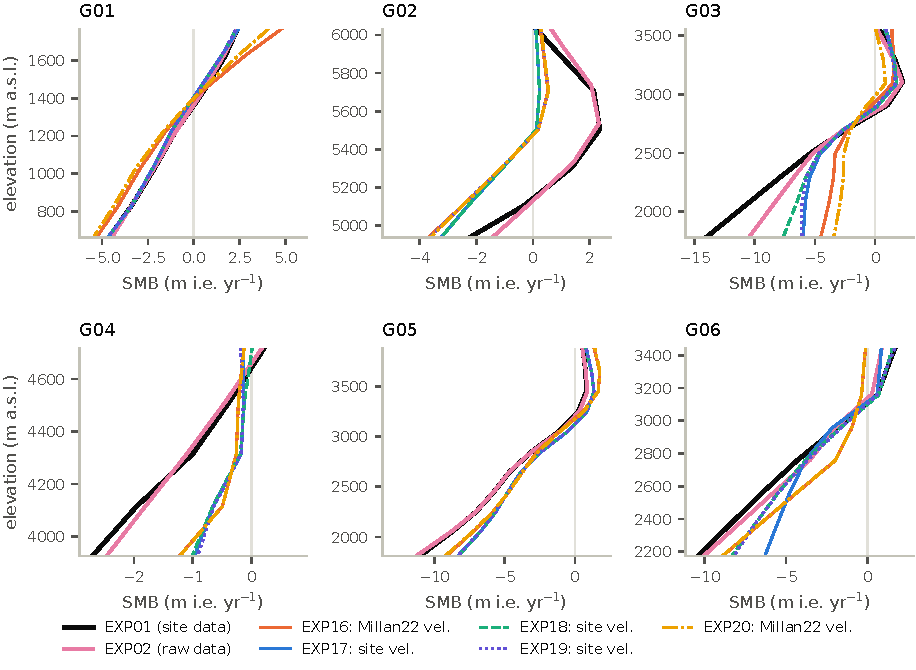
\includegraphics[width=\textwidth]{figures/fig_glob_profiles.pdf}
\caption{Real glaciers: family-mean SMB profiles with site data (EXP01), raw data (EXP02) and globally available inputs
(EXP16--20). EXP17--19 have identical inputs for our method, as have EXP16 and EXP20 on G01, G04 and G06.}
\label{fig:glob}
\end{figure}

\begin{table}[!htb]
\centering
\caption{Raw-data and global-data experiments against EXP01: velocity RMSE (mean observed speed) in \myr, regularisation $\lambda$,
mean thickness and RMS misfit to the independent GPR profiles (m), glacier-wide SMB, modelled / observed mean d$h$/d$t$, ELA (m; -- = no ELA on the
glacier) and mean $\sigma_{\rm SMB}$ (\mie).}
\label{tab:glob}
\resizebox{\textwidth}{!}{\begin{tabular}{llrrrrrrrr}
\toprule
 & & $u_s$ RMSE (mean) & $\lambda$ & $\overline{H}$ & indep.\ GPR & $\overline{\rm SMB}$ & $\overline{{\rm d}h/{\rm d}t}$ mod / obs & ELA & $\overline{\sigma}_{\rm SMB}$ \\
\midrule
G01 & EXP01 & 9.6 (25) & 1000 & 147 & -- & -0.77 & -0.70 / -0.71 & 1361 & 1.15 \\
 & EXP02 (raw data) & 9.3 (25) & 1000 & 144 & -- & -0.78 & -0.73 / -0.73 & 1362 & 1.13 \\
 & EXP16 (Millan22 vel.) & 16.6 (35) & 1000 & 207 & -- & -0.98 & -0.91 / -0.94 & 1389 & 2.56 \\
 & EXP17 (site vel.) & 9.6 (25) & 1000 & 143 & -- & -0.95 & -0.91 / -0.94 & 1401 & 2.37 \\
 & EXP18 (site vel.) & 9.6 (25) & 1000 & 143 & -- & -0.95 & -0.91 / -0.94 & 1401 & 2.37 \\
 & EXP19 (site vel.) & 9.6 (25) & 1000 & 143 & -- & -0.95 & -0.91 / -0.94 & 1401 & 2.37 \\
 & EXP20 (Millan22 vel.) & 14.6 (35) & 300 & 240 & -- & -1.17 & -1.10 / -0.94 & 1497 & 2.74 \\
\midrule
G02 & EXP01 & 3.9 (10) & 100 & 34 & 14 & +1.24 & +1.15 / +1.64 & 5143 & 1.20 \\
 & EXP02 (raw data) & 6.3 (10) & 100 & 28 & 20 & +1.23 & +1.12 / +1.62 & 5130 & 1.22 \\
 & EXP16 (Millan22 vel.) & 3.9 (10) & 100 & 34 & 14 & -0.66 & -0.70 / -0.49 & 5474 & 4.52 \\
 & EXP17 (site vel.) & 7.4 (10) & 1000 & 23 & -- & -0.70 & -0.65 / -0.49 & 5482 & 4.34 \\
 & EXP18 (site vel.) & 7.4 (10) & 1000 & 23 & -- & -0.70 & -0.65 / -0.49 & 5482 & 4.34 \\
 & EXP19 (site vel.) & 3.9 (10) & 100 & 33 & -- & -0.66 & -0.69 / -0.49 & 5475 & 4.50 \\
 & EXP20 (Millan22 vel.) & 4.0 (10) & 100 & 33 & -- & -0.66 & -0.69 / -0.49 & 5475 & 4.51 \\
\midrule
G03 & EXP01 & 9.3 (32) & 100 & 140 & 51 & -0.69 & -1.19 / -0.88 & 2846 & 2.83 \\
 & EXP02 (raw data) & 12.0 (32) & 300 & 130 & 54 & -0.66 & -1.07 / -0.87 & 2856 & 2.61 \\
 & EXP16 (Millan22 vel.) & 13.2 (22) & 1000 & 95 & 135 & -0.56 & -0.84 / -1.06 & 2934 & 3.77 \\
 & EXP17 (site vel.) & 9.3 (32) & 100 & 130 & -- & -0.67 & -1.29 / -1.06 & 2884 & 4.02 \\
 & EXP18 (site vel.) & 9.3 (32) & 100 & 130 & -- & -0.72 & -1.30 / -1.06 & 2885 & 4.04 \\
 & EXP19 (site vel.) & 9.3 (32) & 100 & 130 & -- & -0.74 & -1.34 / -1.06 & 2888 & 4.01 \\
 & EXP20 (Millan22 vel.) & 12.9 (22) & 300 & 69 & -- & -0.79 & -1.06 / -1.06 & 2988 & 3.60 \\
\midrule
G04 & EXP01 & 2.6 (3) & 100 & 28 & -- & -1.29 & -1.21 / -1.30 & 4642 & 0.52 \\
 & EXP02 (raw data) & 5.2 (5) & 300 & 9 & -- & -1.27 & -1.04 / -1.30 & 4659 & 0.49 \\
 & EXP16 (Millan22 vel.) & 13.1 (9) & 100 & 12 & -- & -0.41 & -0.39 / -0.42 & -- & 1.80 \\
 & EXP17 (site vel.) & 2.6 (3) & 100 & 28 & -- & -0.39 & -0.39 / -0.42 & 4632 & 1.85 \\
 & EXP18 (site vel.) & 2.6 (3) & 100 & 28 & -- & -0.39 & -0.39 / -0.42 & 4609 & 1.85 \\
 & EXP19 (site vel.) & 2.6 (3) & 100 & 28 & -- & -0.39 & -0.39 / -0.42 & -- & 1.85 \\
 & EXP20 (Millan22 vel.) & 13.1 (9) & 100 & 12 & -- & -0.41 & -0.38 / -0.42 & -- & 1.80 \\
\midrule
G05 & EXP01 & 12.1 (41) & 300 & 161 & 65 & -1.93 & -2.04 / -1.95 & 3216 & 2.32 \\
 & EXP02 (raw data) & 11.3 (41) & 300 & 159 & 70 & -1.90 & -2.07 / -1.95 & 3205 & 2.35 \\
 & EXP16 (Millan22 vel.) & 10.8 (47) & 300 & 171 & 78 & -1.21 & -1.37 / -1.29 & 3183 & 3.51 \\
 & EXP17 (site vel.) & 10.5 (41) & 100 & 169 & -- & -1.17 & -1.39 / -1.29 & 3128 & 3.73 \\
 & EXP18 (site vel.) & 10.5 (41) & 100 & 169 & -- & -1.17 & -1.40 / -1.29 & 3127 & 3.73 \\
 & EXP19 (site vel.) & 10.5 (41) & 100 & 169 & -- & -1.16 & -1.39 / -1.29 & 3127 & 3.73 \\
 & EXP20 (Millan22 vel.) & 8.9 (47) & 100 & 180 & -- & -1.19 & -1.40 / -1.29 & 3175 & 3.78 \\
\midrule
G06 & EXP01 & 24.1 (31) & 100 & 117 & -- & -0.87 & -0.87 / -0.96 & 3109 & 1.71 \\
 & EXP02 (raw data) & 21.7 (27) & 600 & 90 & -- & -1.07 & -0.96 / -0.95 & 3137 & 1.18 \\
 & EXP16 (Millan22 vel.) & 14.1 (12) & 300 & 54 & -- & -0.95 & -0.82 / -0.79 & -- & 1.36 \\
 & EXP17 (site vel.) & 29.4 (31) & 600 & 92 & -- & -0.90 & -0.83 / -0.79 & 3114 & 1.81 \\
 & EXP18 (site vel.) & 24.1 (31) & 100 & 118 & -- & -0.68 & -0.71 / -0.79 & 3102 & 2.18 \\
 & EXP19 (site vel.) & 24.1 (31) & 100 & 117 & -- & -0.68 & -0.71 / -0.79 & 3106 & 2.18 \\
 & EXP20 (Millan22 vel.) & 14.1 (12) & 300 & 54 & -- & -0.96 & -0.83 / -0.79 & -- & 1.36 \\
\bottomrule
\end{tabular}
}
\end{table}

%=====================================================================================================================
\section{Discussion and open points}\label{sec:open}
\begin{itemize}\setlength{\itemsep}{1pt}
\item \textbf{Thickness without observations.} Where no GPR exists (S01, G01, G04, G06) the thickness, and hence FDIV,
depends on the first guess. On S01 this leads to a 1.0\,\mie\ FDIV bias although the SMB itself is well recovered.
\item \textbf{GPR.} The cross-validated weight keeps the GPR from being trusted beyond its accuracy, but the
information gain away from the profiles is small ($\le$\,3\,\% on withheld profiles). A stronger spatial propagation
would need a different prior (e.g.\ a correlation length in $R$), which would give the profiles exactly the excess
weight the cross-validation avoids.
\item \textbf{Resolution.} Grids coarser than $\sim$100\,m (EXP14 S02, EXP15 S01) break the forward model. Running the
model on a refined grid interpolated from the coarse input is the obvious remedy.
\item \textbf{L-curve.} The automatic L-curve corner is not always reproducible (G06: EXP17 against EXP18; G01: EXP16
against EXP20).
Taking $\lambda$ from EXP01 for every experiment of a glacier, or averaging the SMB over neighbouring $\lambda$, would
remove this source of scatter, at the cost of re-running the affected experiments.
\item \textbf{Elevation change of G02.} The d$h$/d$t$ of G02 in EXP01 and in the raw data (+1.64 and +1.62\,\myr) disagrees
in sign with \citet{hugonnet} ($-0.49$); to be raised with the organisers.
\item \textbf{Velocity coverage.} On S02 the raw data leave the upper glacier without velocities and the ELA drops by
500\,m, while the glacier-wide SMB is unchanged. Glacier-wide numbers alone hide such failures; the stake comparison of
the organisers will be the real test.
\item \textbf{Status.} All runs except EXP14 for G01 are complete. EXP14 for G01 runs on a 75\,m grid with 149\,000 ice
cells; its estimated memory (24\,GB) exceeds that of one RTX\,4090, so the scheduler cannot start it. It needs a larger
GPU, a direct attempt on an otherwise empty card, or a coarser model grid; the choice is pending.
\end{itemize}

\begin{thebibliography}{99}\small
\bibitem[ContinuIX(2026)]{continuix} ContinuIX working group: Protocol for work packages 2 and 3, \url{https://github.com/ContinuIX/ContinuIX-1}; data: \url{https://doi.org/10.5281/zenodo.21401808}, 2026.
\bibitem[Jouvet et al.(2026)]{igm} Jouvet, G., Finley, B., Gregov, T., and Rosier, S.: IGM: an accessible, modular, differentiable, and GPU-accelerated high-order ice flow model, EarthArXiv, \url{https://doi.org/10.31223/X5GB6G}, 2026.
\bibitem[Lleshi et al.(submitted)]{lleshi} Lleshi, K., Jouvet, G., Kneib, M., Gregov, T., and Herman, F.: Surface mass balance inference based on a transient glacier evolution model inversion, The Cryosphere, submitted.
\bibitem[Farinotti et al.(2019)]{farinotti} Farinotti, D., Huss, M., F\"urst, J.\,J., Landmann, J., Machguth, H., Maussion, F., and Pandit, A.: A consensus estimate for the ice thickness distribution of all glaciers on Earth, Nat. Geosci., 12, 168--173, 2019.
\bibitem[Hugonnet et al.(2021)]{hugonnet} Hugonnet, R., McNabb, R., Berthier, E., et al.: Accelerated global glacier mass loss in the early twenty-first century, Nature, 592, 726--731, 2021.
\bibitem[Millan et al.(2022)]{millan} Millan, R., Mouginot, J., Rabatel, A., and Morlighem, M.: Ice velocity and thickness of the world's glaciers, Nat. Geosci., 15, 124--129, 2022.
\bibitem[Hansen(1998)]{hansen} Hansen, P.\,C.: Rank-Deficient and Discrete Ill-Posed Problems: Numerical Aspects of Linear Inversion, SIAM, Philadelphia, 1998.
\bibitem[Akiba et al.(2019)]{optuna} Akiba, T., Sano, S., Yanase, T., Ohta, T., and Koyama, M.: Optuna: a next-generation hyperparameter optimization framework, Proc. 25th ACM SIGKDD, 2623--2631, 2019.
\end{thebibliography}

\appendix
\section{Synthetic results per experiment}
\begin{table}[H]
\centering
\caption{All synthetic runs. Left: S01; right: S02. SMB RMSE against the prescribed law (S01); $\overline{\rm SMB}$
glacier-wide SMB and $\overline{\dot h}_{\rm mod}$ modelled mean d$h$/d$t$ (\mie); $H$ RMSE against the true EXP01
thickness (m); GPR c.-v. = RMS misfit (m) to that experiment's (possibly perturbed) cross-validation GPR profile. S01 is not part of
EXP02. $^\dagger$\,Forward model fails on the coarse grid (Sect.~\ref{sec:sens}).}
\label{tab:synall}
\resizebox{\textwidth}{!}{\begin{tabular}{l|rrrrrr|rrrrrr}
\toprule
 & $\tau_{\rm ref}$ & $A$ & SMB RMSE & $\overline{\rm SMB}$ & $\overline{\dot h}_{\rm mod}$ & $H$ RMSE & $\tau_{\rm ref}$ & $A$ & $\overline{\rm SMB}$ & $\overline{\dot h}_{\rm mod}$ / obs & $H$ RMSE & GPR c.-v. \\
\midrule
EXP01 & 1.877 & 30 & 0.67 & -0.00 & -0.90 & 58 & 0.073 & 119 & -0.17 & -0.53 / -0.42 & 51 & 50 \\
EXP02 & n/a & n/a & n/a & n/a & n/a & n/a & 0.664 & 119 & -0.13 & -0.47 / -0.42 & 93 & 90 \\
EXP03 & 1.873 & 30 & 0.71 & -0.01 & -0.91 & 58 & 0.149 & 120 & -0.17 & -0.53 / -0.42 & 51 & 42 \\
EXP04 & 1.822 & 30 & 0.68 & +0.00 & -0.90 & 57 & 0.219 & 120 & -0.17 & -0.53 / -0.42 & 52 & 70 \\
EXP05 & 1.774 & 30 & 0.57 & +0.06 & -0.87 & 59 & 0.127 & 120 & -0.15 & -0.56 / -0.44 & 51 & 37 \\
EXP06 & 1.873 & 30 & 0.67 & +0.01 & -0.89 & 58 & 0.097 & 120 & -0.17 & -0.53 / -0.42 & 51 & 142 \\
EXP07 & 1.822 & 30 & 0.67 & +0.01 & -0.89 & 57 & 0.071 & 119 & -0.18 & -0.54 / -0.42 & 52 & 97 \\
EXP08 & 1.956 & 31 & 0.54 & +0.02 & -0.89 & 58 & 1.645 & 120 & -0.16 & -0.51 / -0.42 & 53 & 55 \\
EXP09 & 1.805 & 85 & 1.29 & -0.08 & -0.79 & 34 & 0.111 & 120 & -0.17 & -0.56 / -0.42 & 57 & 51 \\
EXP10 & 1.956 & 30 & 0.68 & -0.02 & -0.91 & 58 & 1.223 & 119 & -0.17 & -0.54 / -0.42 & 52 & 52 \\
EXP11 & 1.698 & 30 & 0.66 & -0.01 & -0.90 & 57 & 1.645 & 119 & -0.17 & -0.53 / -0.42 & 51 & 51 \\
EXP12 & 1.883 & 88 & 1.18 & -0.03 & -0.91 & 42 & 0.071 & 119 & -0.18 & -0.52 / -0.42 & 54 & 50 \\
EXP13 & 1.792 & 30 & 0.61 & +0.02 & -0.90 & 62 & 0.071 & 119 & -0.10 & -0.63 / -0.42 & 64 & 50 \\
EXP14$^\dagger$ & 0.437 & 85 & 1.07 & -0.18 & -0.77 & 30 & 0.070 & 119 & +3.36 & -2.31 / -0.41 & 132 & 235 \\
EXP15$^\dagger$ & 0.050 & 119 & 28.20 & +26.54 & -4.51 & 100 & 0.070 & 119 & -0.17 & -0.53 / -0.42 & 51 & 51 \\
\bottomrule
\end{tabular}
}
\end{table}

\end{document}
